%
% fig-rand.tex
%
% (c) 2025 Prof Dr Andreas Müller
%
\begin{figure}
\centering
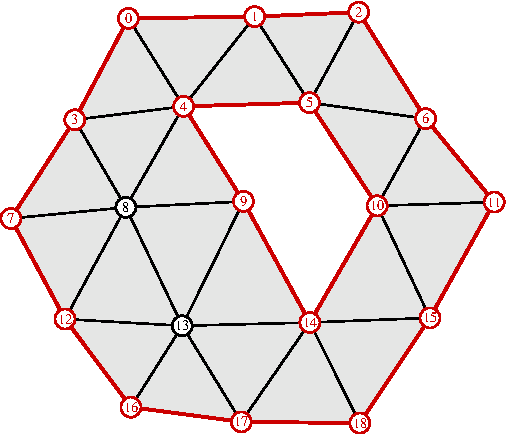
\includegraphics{chapters/120-topologie/images/rand.pdf}
\caption{Rand eines zweidimensionalen Zellenkomplexes.
\index{Rand}
Die schwarzen Kanten sind innere Kanten und gehören nicht zum Rand.
Nur Kanten, die zu nur einem 2-Simplex gehören, tragen zum Rand bei.
\label{buch:topologie:homologie:fig:rand}}
\end{figure}
